\documentclass[bachelor,english]{info1thesis}
% Mögliche Parameter für den Typ der Arbeit:
% - bachelor: Bachelorarbeit
% - master: Masterarbeit
\usepackage[utf8]{inputenc}
\usepackage[T1]{fontenc}
\usepackage{algorithm2e}
\usepackage{tikz}
\usepackage{listings}
\usepackage{color}
\usepackage[onehalfspacing]{setspace}
\usepackage{graphicx}
\usepackage{textcomp}

\definecolor{codegreen}{rgb}{0,0.6,0}
\definecolor{codegray}{rgb}{0.5,0.5,0.5}
\definecolor{codepurple}{rgb}{0.58,0,0.82}
\definecolor{backcolour}{rgb}{0.95,0.95,0.92}

\lstdefinestyle{arff}{
	backgroundcolor=\color{backcolour},
	commentstyle=\color{codegreen},
	keywordstyle=\color{blue},
	keywordstyle={[2]\color{magenta}},
	numberstyle=\tiny\color{codegray},
	stringstyle=\color{codepurple},
	basicstyle=\footnotesize,
	comment=[l]{\%},
	keywords={@relation,@attribute,@data},
	morekeywords=[2]{real,integer,numeric,string,date},
	breakatwhitespace=false,
	breaklines=true,
	captionpos=b,
	keepspaces=true,
	numbers=left,
	numbersep=5pt,
	showspaces=false,
	showstringspaces=false,
	showtabs=false,
	tabsize=2
}

\lstset{style=arff}



%%% Titelseite -- hier Titel und Autorennamen eintragen
% Geben Sie hier den Titel Ihrer Arbeit an.
\title{Extraction and preprocessing of heating systems data for declarative data mining}
% Geben Sie Ihren Namen an.
\author{Fatih Kesikli}
% Abgabedatum kann modifiziert werden (in englischer Schreibweise angeben)
\date{May 07, 2020}
% Hier zusätzlich noch das Datum in deutscher Sprache angeben
\germandate{May 07, 2020}
% Betreuer eintragen
\supervisors{Prof.\ Dr.\ Dietmar Seipel\and
Daniel Weidner, M.\,Sc.}



\begin{document}
%%%%%%%%%%%%%%%%%%%%%%%%%%%%%%%%%%%%%%%%%%%%%%%%%%%%%%%%%%%%%%%%%%%%%%%%%%








%%%%%%%%%%%%%%%%%%%%%%%%%%%%%%%%%%%%%%%%%%%%%%%%%%%%%%%%%%%%%%%%%%%%%%%%%%%%%%%%
%%% Abstract
\begin{abstract}
    With data mining being a widely popular tool in extracting knowledge out of large databases, data preprocessing is often a major and necessary but neglected step. In this study, data mining will be applied on a specific set of heating systems data represented as CSV-files, using WEKA and Declare. The data sets represent each 20000 measurements of generators, heating, and hotwater CSV-files provided by ENER-IQ. An attempt at finding useful preprocessing parameters is shown, mostly leaning on Equal-Width-Discretization. While the output rules are often redundant and vague, a rough overview of the given heating system can be extracted, which is an improvement over no preprocessing.	
\end{abstract}
\begin{germanabstract}
	In dieser Arbeit wird mit Hilfe der Frameworks WEKA und Declare ein Versuch an der Extraktion von Wissen aus gegebenen Heizungsdaten in Form von CSV-Dateien dargestellt. Die gegebenen Heizungsdaten repräsentieren pro CSV-Datei jeweils 20000 Messungen eines Generators, Heizkörpers oder Warmwassersystem und ist bereitgestellt von ENER-IQ. Das hauptsächliche Interesse dieser Arbeit ist das Vorverarbeiten der Heizungsdaten, sodass Data Mining sinnvoll angewandt werden kann. Das Vorverarbeiten der CSV-Dateien basiert hauptsächlich auf Equal-Width-Discretization. Obwohl die vorgestellten Ergebnisse triviales Wissen über die gegebenen Heizungssysteme darstellen, helfen sie dennoch grobe Fehler in einem Heizungssystem aufzuweisen und geben eine sinnvolle erste Einschätzung.
\end{germanabstract}

\thesistableofcontents





%%%%%%%%%%%%%%%%%%%%%%%%%%%%%%%%%%%%%%%%%%%%%%%%%%%%%%%%%%%%%%%%%%%%%%%%%%%%%%%%
\chapter{Introduction}
\label{sec:introduction}

With climate change potentially being one of the biggest threats \cite{bickton2016climate} to our planet of our time, different fields in engineering are suggesting various coping mechanisms. One common approach is to reduce emissions in household goods or households. Extending on this idea, one of the motivations of this thesis is potentially finding correlations in heating systems that would help save energy and ultimately reduce carbon emissions. Unlike traditionally, this approach is not focused on the engineering of heating systems, but rather on finding correlations of measurements in heating systems through data mining. The hypothesis here is that applying a data mining process on a given set of measurements should help configuring parameters of that heating system in order to e.g. reduce emissions.

Apart from reducing emissions, another motivation and common application of data mining and data science is diagnosing faults in machines, such as shown by Nauro et al. \cite{naruo1990development}. Often times, the largest effort into repairing malfunctions in machines is diagnosing the malfunction. Therefore it is of interest to speed up the diagnosing process in order to save costs and valuable production time and uptime.

This thesis is leaned on the work of sustainability engineers such as from ENER-IQ, a company that uses artificial intelligence approaches to reduce costs, energy, and emissions in client heating systems - the company that also provided the measurements this thesis is based on. Unlike ENER-IQ, a smaller scale declarative data mining approach with different frameworks is used, unlike the e.g. deep learning approaches used by the former.

Chapter \ref{sec:fundamentals} discusses all necessary terms and concepts used in this paper's approach, chapter \ref{sec:relatedwork} illustrates the differences between similar research and projects, chapter \ref{sec:approach} is an overview of the most important steps in execution of the used approach, chapter \ref{sec:implementation} walks through various implementations used, chapter \ref{sec:evaluation} discusses evaluations of the aforementioned experiments, chapter \ref{sec:futurework} is concerned with shortcomings and lessons to be learned from this study, and finally chapter \ref{sec:summary} summarizes the results of the most important evaluations.






%%%%%%%%%%%%%%%%%%%%%%%%%%%%%%%%%%%%%%%%%%%%%%%%%%%%%%%%%%%%%%%%%%%%%%%%%%%%%%%%
%\section{Definitions}
%\label{sec:definitions}
%Evtl. nicht notwendig





%%%%%%%%%%%%%%%%%%%%%%%%%%%%%%%%%%%%%%%%%%%%%%%%%%%%%%%%%%%%%%%%%%%%%%%%%%%%%%%%


\chapter{Fundamentals}
\label{sec:fundamentals}
This chapter introduces the concepts necessary to for one understand related work in the field of association rule mining and secondly to follow the reasoning behind the evaluations of the experiments conducted in chapter \ref{sec:evaluation}. 

\section{Declarative Data Mining}
\label{sec:datamining}
According to Bissantz et al., the term data mining roughly surrounds the concept of extracting knowledge from vast amounts of data that is implicitly hidden \cite{bissantz2009data}. Declarative data mining then refers to using declarative tools to practice data mining. Blockeel and Hendrick claim that introducing declarative techniques to data mining may solve the issue of misusing and misinterpreting data mining strategies by focusing on describing the underlying data analysis problem instead of describing the method to solve the problem. In other fields of computer science, declarative programming languages have proven to be useful as well, mostly in software engineering, where the declarative concepts have been used to increase robustness and enable easier debugging of software systems. For example, procedural languages such as Java have adopted declarative designs, such as lambda notations, and functional (which is a subtype of declarative) languages such as Haskell have experienced a rise in popularity in the last couple of years \cite{blockeel2015data}.

In this case, the declarative tool being used is the programming language Prolog in combination with the declarative framework Declare. The latter provides a Prolog API for the WEKA framework, which implements a collection of artificial intelligence and data mining algorithms. \newline


\subsection{Association Rule Mining}
\label{sec:associationrulemining}

In data mining research, one of the most popular methods of extracting knowledge out of databases is \textit{Association Rule Mining}, according to Liu et al. \cite{liu1998integrating}. More precisely, the goal of Association Rule Mining is gathering relationships between items of many transactions stored in a database.

Furthermore, Liu et al. provide a formally laid out description of the Association Rule Mining problem:\newline

\begin{definition}
Let $I = {x_1, ..., x_n}$ be a set of distinct literals, called items. A set $X \subseteq I$ with $k = |X|$ is called a \textit{k}-itemset or simply an itemset. Let a database \textit{D} be a multi-set [a set that allows multiple occurrences of the same element] of subsets of $I$. Each $T \in D$ is called a transaction. We say that a transaction $T \in D$ supports an itemset $X \in I$ if $X \in T$ holds.\newline
\end{definition}


Having defined the database at hand, Liu et al. further define \textit{association rules}, which are the results to be obtained:\newline



\begin{definition}
An association rule is an expression $X \Rightarrow Y$, where $X, Y$ are itemsets and $X \cap Y = \emptyset$ holds.\newline
\end{definition}



The most popular introductory example in literature to association rule mining is the studying of \textit{Market Basket Analysis}. Most retailers are interested in consumer behavior in order to more effectively target their advertisements to customers, position their items, or offer discounts. In this case, our itemsets from the definition above are represented as a list of items, as in e.g. groceries, a customer bought together, such as ${beer, cheese, potato chips, apples}$. Association rules here would be any implication between arbitrary subsets, e.g. ${beer, potato chip} \Rightarrow {cheese}$. The database would consist of all recordings of items bought together by a customer.\newline
This example itself shows a problem to be addressed: Any itemset allows for an exponential amount of association rules to be generated. Therefore, additional metrics have to be introduced, such as \textit{support} and \textit{confidence}, as will be in section \ref{sec:apriori}.

\subsection{Finding frequent item sets with Apriori}
\label{sec:apriori}

Section \ref{sec:associationrulemining} explained the need for additional metrics to filter association rules.

The support metric for itemsets describes for each itemset its proportion in which it appears in all transactions of a database. In other words, the support metric is the popularity of an itemset in a database.
Given an itemset $I = {A_1, ..., A_n}$, its support is defined as

	\vspace{0.2cm}
\[supp(I) = P(A_1, ..., A_n)\]
	\vspace{0.2cm}

The same can be defined for association rules, which is deducted from the support for item sets:

	\vspace{0.2cm}
\[supp(X \Rightarrow Y) = \frac{supp(X \cup Y)}{N},\]
	\vspace{0.2cm}

where \textit{X,Y} are item sets and \textit{N} is the amount of transactions, where \textit{X} or \textit{Y} is a member of.

Another metric in Apriori used to filter item sets is \textit{confidence}. The confidence metric is used to filter association rules, where the implication under a given premise is not supported often enough. This allows to exclude association rules that represent outliers in a given database. 

Due to the exponential amount itemsets in a given database, a naive implementation iterating through all possible itemsets and counting their frequency is unreasonable.
First introduced in 1994 by Agrawal et al. \cite{agrawal1994fast}, Apriori is a specific implementation of an algorithm to find frequent itemsets as specified in the previous section. Unlike the mentioned naive implementation, Apriori makes use of the Apriori property:

\begin{definition}
	\vspace{0.5cm}
	All subsets of a frequent itemset must be frequent.
	If an itemset is infrequent, all its supersets will be infrequent.
	\vspace{0.5cm} 
\end{definition}	

Abusing this property, the Apriori algorithm prunes non relevant itemsets and further filters itemsets by testing them against the parameterized minimum support. The minimum confidence metric is used when generating association rules out of the extracted frequent itemsets. This is done by the subroutine \textit{apriori-gen}.

The following algorithm as illustrated by Ye et al. \cite{ye2006parallel} combines both extracting frequent itemsets with Apriori and generating association rules with apriori-gen. The algorithm starts with 1-itemsets which uphold the required minimum support requirement. This process is called \textit{pruning}. Afterwards, the frequent 1-itemsets are joined into 2-itemsets, where pruning is again applied to filter non frequent itemsets. This routine is continued until k+1-itemset does not return new candidates. 

   \begin{algorithm}
	\SetAlgoLined
	\KwIn{Database $DB$, minimum support $minsup$}
	\KwOut{Frequent itemsets $L_i$}
	Get $L_1$ for 1-itemsets;\newline
	k = 2;\newline
	\While{$L_(k-1)$ <> empty}
	{
		$C_k$ = Apriori-gen($L_(k-1)$);
		
	}
	\For{Transaction $T$ : $DB$}
	{
		\For{Itemset $c$ : $C_k$}
		{
			\If{$T$ includes $c$}
			{
				count[c]++;
			}
		}
	}
	$L_k$ = prunecandidate($C_k$, $minsup$);
	$k$++;
	\KwResult{$L_1,...,L_k$}
	\caption{Apriori algorithm using Apriori-gen and pruning}
	\label{alg:apriori}
	%\vspace{1cm}
\end{algorithm}

The above algorithm calls subroutines $prunecandidate$ to test itemsets against the required minimum support and $apriori-gen$ to generate association rules, as further defined by Yet et al.:

   \begin{algorithm}
	\SetAlgoLined
	\KwIn{Frequent itemset $L_(k-1)$ }
	\KwOut{Set of candidate itemsets $C_k$}
	\For{Itemset $m$ : $L_(k-1)$}
	{
		\For{Itemset $n$ : $L_(k-1)$}
		{
			\If{$m$ <> n}
			{
				$l$ = $m$ join $n$;
				\If{sizeof($l$) == k}
				{
					$C_k$ = $C_k \cup l$;
				}
			}
		}
	}
	\KwResult{$C_k$}
	\caption{Apriori-gen subroutine called by apriori algorithm}
	\label{alg:apriorigen}
	%\vspace{1cm}
\end{algorithm}


   \begin{algorithm}
	\SetAlgoLined
	\KwIn{Set of candidate itemsets $C_k$, minimum support $minsupp$}
	\KwOut{Frequent itemset $L_k$}
	\For{Itemset $c$ : $C_k$}
	{
	\If{$support(c) >= minsupp$}
	{
		$L_k$ = $L_k \cup c$
	}
	}
	\KwResult{$L_k$}
	\caption{prunecandidate}
	\label{alg:aprioriprune}
	%\vspace{1cm}
\end{algorithm}






%\cite{palancar2008compressed}



%\cite{agrawal1993mining}

\subsection{Mining association rules with WEKA-Apriori}
\label{sec:wekaapriori}

While the last section discussed the Apriori algorithm and the usage of metrics such as support and confidence to prune candidate itemsets, this section is concerned with a specific Apriori implementation provided by the WEKA framework. This framework will later be used in chapter \ref{sec:evaluation} in order to extract association rules.
WEKA \cite{hall2009weka} is a popular open source machine learning tool written in Java by the University of Waikato. Besides many other functionalities, here specifically its association rule mining purposes are of interest. One example process and application of WEKA for extracting association rules is demonstrated by Srivastava et al. \cite{srivastava2014weka}.

The core to mining association rules using the WEKA tool is the underlying implementation of the Apriori algorithm. In literature, there are different implementations of Apriori, often differing in the usage of parameters, usage of data structures for performance reasons, optimized subroutines etc. . Traditionally, Apriori takes parameters specifying the minimum support and minimum confidence each association rule is supposed to uphold. WEKA's Apriori implementation's main difference consists of taking in the minimum amount of association rules to mine instead of a minimum support parameter. This works, because the parameter specifying the required amount of rules implicates the required minimum support to do so. WEKA does this by iteratively executing a traditional version of Apriori that takes in lower minimum support parameter each execution until an iteration is able to reach the specified amount of rules, as is explained in WEKA's documentation.

Besides minimum support and minimum confidence, WEKA's documentation \cite{agrawal1994fast} further specifies an array of different parameters. Some of the for this application deemed important and later used in section \ref{sec:evaluation} are:

\vspace{0.4cm}

\begin{description}
	\item[N]\hfill \\
	Required amount of rules, which implicitly determines the minimum support required.
	\item[C]\hfill \\ 
	Minimum Confidence used in the prune phase.
	\item[D]\hfill \\ 
	Since a traditional version of Apriori is executed after every iteration with a lower minimum support value, this parameter specifies the step by which to lower the minimum support after each iteration. The default value is 0.05.
	\item[T]\hfill \\ 
	This parameter allows to sort the extracted rules by the specified metric. Metrics to specify are either confidence, lift, leverage, or conviction. The usage of this parameter allows for a more readable output of association rule. This is relevant, since in association rule mining it is often humans parsing results, unlike in other artificial intelligence approaches.\newline If the amount of extractable rules exceeds the amount of required rules specified by the -N parameter, this parameter makes a difference in which rules are output or filtered.
	
	\item[I]\hfill \\ 
	Also for readability purposes, this parameter prints out additional header information in the output file by naming all found itemsets instead of only listing all rules. This does not influence the extracted rules.
		
\end{description}

Further parameters allowed by WEKA, however not used in this work, are

\begin{description}
	\item[U and M]\hfill \\
	Respectively upper (-U) and lower (-M) bounds for minimum support. Rules exceeding these bounds are not considers in the extracted association rules.
	\item[R]\hfill \\ 
	Allows for a form of preprocessing by pruning every transaction that contains attributes which are unspecified. This is not the case for any of the given heating data.
	
\end{description}


First, the database at hand has to be represented as an ARFF-file. ARFF (Attribute Relation File Format) is a format specifically designed as an input file for the WEKA tool and is specified in its documentation \cite{docarff}. 

Listing \ref{lst:examplearff} by the University of Waikato illustrates an example ARFF file.
Every ARFF-file consists of a header and the main data. The header provides information regarding the relation name and its attributes (columns). Each attribute is declared beginning with the keyword \textit{@ATTRIBUTE}, followed by the attribute's name and the type of data that attribute represent. Accepted data types are e.g. \textit{NUMERIC}, \textit{date}, or \textit{NOMINAL}. Alternatively to its data type, the user can specify the attribute's value range directly. In this work the latter will be the case, as will be part of the discussion later in section \ref{sec:evaluation}. \newline The main data of a relation is declared after the keyword \textit{@DATA}, where the data is represented similar to a CSV-file. \newline
All heating data CSV-files have to be converted into ARFF-file in order to apply WEKA Apriori. This will be done with the help of the Declare framework in Prolog.

\vspace{0.2cm}

\begin{figure}
\begin{lstlisting}[style=arff, caption= Example ARFF file \cite{docarff}, label={lst:examplearff}]

% 1. Title: Iris Plants Database
% 
% 2. Sources:
%      (a) Creator: R.A. Fisher
%      (b) Donor: Michael Marshall (MARSHALL%PLU@io.arc.nasa.gov)
%      (c) Date: July, 1988
% 
@RELATION iris

@ATTRIBUTE sepallength  NUMERIC
@ATTRIBUTE sepalwidth   NUMERIC
@ATTRIBUTE petallength  NUMERIC
@ATTRIBUTE petalwidth   NUMERIC
@ATTRIBUTE class        {Iris-setosa,Iris-versicolor,Iris-virginica}

@DATA
5.1,3.5,1.4,0.2,Iris-setosa
4.9,3.0,1.4,0.2,Iris-setosa
4.7,3.2,1.3,0.2,Iris-setosa
4.6,3.1,1.5,0.2,Iris-setosa
5.0,3.6,1.4,0.2,Iris-setosa
5.4,3.9,1.7,0.4,Iris-setosa
4.6,3.4,1.4,0.3,Iris-setosa
5.0,3.4,1.5,0.2,Iris-setosa
4.4,2.9,1.4,0.2,Iris-setosa
4.9,3.1,1.5,0.1,Iris-setosa

\end{lstlisting}
\end{figure}
\vspace{0.2cm}



\section{Heating Circuits}
\label{sec:heatingcircuits}
The purpose of this chapter is not to thoroughly dive into the engineering behind heating circuits, but to provide knowledge about heating circuits that is required to follow the reasoning behind the chosen preprocessing strategies and the evaluation in chapter \ref{sec:evaluation}.

\subsection{Components} 
\label{sec:components}

Any given heating circuit consists of at least a heating source, a radiation unit, and flow/return pipes.


Common heating sources (or generators) are furnaces, heat pumps, or boilers. Depending on which heating source is used, we might have different expectations for our measurements. For example, furnaces using gas or oil as fuel commonly have a higher energy efficiency (despite their emissions), while boilers tend to have lower energy efficiency. This knowledge is necessary when one were to compare e.g. consumed energy in the heating source and the provided room temperature by the radiation unit. In the case of furnaces, another point to factor into energy efficiency is the kind of fuel that is used. Another point to note is that one heating source can distribute heating energy to multiple radiators. This type of heating system is called \textit{central heating}. This information could be useful when determining error sources. For example, when observing a lower room temperature at given radiators, which share the same heating source, one might to further observe the heating source for potential faults.
Another point of interest are exhaust pipes, since steam and gas are produced by e.g. combustion in the furnace. Energy expended and wasted through exhaust pipes is a  possible deficiency and fault causes for heating sources.



The energy generated by the heating source is then transferred to radiation units which ultimately expend their energy over their surface. As with the heating source, multiple variables affect the amount of energy radiated, such as material, amount of panels, surface area, etc. 

The pipes transferring hot water towards the radiators are called flow pipes, whereas the pipes returning cooled down water, after the radiator expended as much energy possible, are called return pipes. The returned cooled down water is then reused in the heating source, where the cycle enters its next iteration.

Sometimes circulating pipes and pumps are used to keep hotwater in motion. This allows hotwater to not expend its energy while it is "waiting" in the pipes when it is not used by the radiator.

\subsection{Measurements}
\label{sec:measurements}

The following provides a brief description of all measured units:

\begin{description}
	\item[Vorlauf (flow temperature)]\hfill \\
	Measurement of temperature of water in the flow pipe in Degree Celsius. This measurement is listed in both generator and radiator CSV-files. The difference between flow temperature measurement for generator and radiator is the specific location at where the sensor is located.
	\item[Rücklauf (return temperature)]\hfill \\ 
	Measurement of temperature of water in the return pipe after cooling down in Degree Celsius. Analog to \textit{Vorlauf}.
	\item[Warmwaser (hotwater)]\hfill \\ 
	Measurement of temperature in the hotwater pipe in Degree Celsius.
	\item[Zirku (circulation temperature)]\hfill \\ 
	Measurement of temperature in the circulating pipe in Degree Celsius.
	
	\item[Abgas (exhaust temperature)]\hfill \\ 
	Measurement of exhaust pipe temperature in Degree Celsius.
	\item[Spreizung (flow temperature - return temperature)]\hfill \\ 
	Difference between flow and return temperature in Kelvin. This attribute is not a sensor measurement and was generated artificially.
	\item[Uhrzeit (date and time)]\hfill \\ 
	Date and time of each measurement in ISO-8601 format.
	
\end{description}





\section{Preprocessing of CSV-data}
\label{sec:preprocessing}
All heating circuit data provided by ENER-IQ GmbH \cite{eneriq}, a startup company dedicated to optimize usage of resources in heating systems in order to reduce costs and environmental damage done, is represented in CSV-files. Each of the three groupings (Generator, Heating, Hotwater) contain 2-3 different CSV-files. All CSV-files in a given grouping represent the same columns, which however differ between the groups. Chapter \ref{sec:heatingcircuits} further discusses the semantics and how to interpret the data at hand.

The necessity to preprocess our data comes from the fact that using raw sensor data to mine association rules results in no rules since the underlying WEKA-Apriori algorithm is not able to find frequent itemsets. This is due to sensors returning continuous data, mostly temperatures in multiple digits after the comma. Therefore the cardinality of any given column is on a similar scale to the amount of records presented in the representing CSV-file. 
In order to find appropriate preprocessing strategies for this specific data of heating systems, we have to look into the data types of our measured data (e.g. whether a column represents an integer, string values etc.).

This chapter's main focus is to discuss strategies to preprocess the provided data in a way to extract association rules through the WEKA-framework between the measured items later in chapter \ref{sec:evaluation}. Furthermore, an on of an early framework in Java/Prolog, which is also used in \ref{sec:evaluation}, will be suggested.

\subsection{Types of data}
\label{typesofdata}
Since different preprocessing techniques apply for different types of data, we have to establish a terminology regarding the unique characteristics of types of data.

In data science literature, there are multiple terminologies to distinguish between. Here, the terminology of Yang et al. (\cite{yang2009discretization}) is used.
Looking into the heating data from tables \ref{table:generator}, \ref{table:heating}, \ref{table:hotwater}, the data can be split into different categories, according to Yang et al, as illustrated in figure \ref{fig:typesofdata}:

\begin{figure}
	\centering
	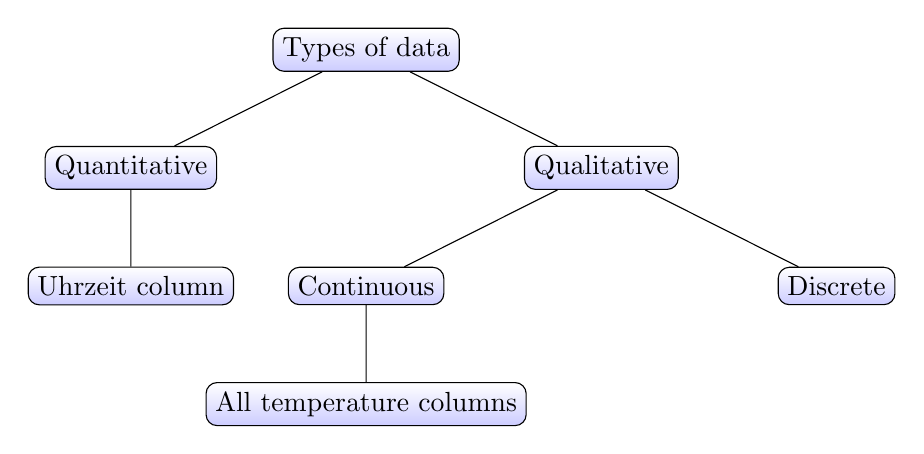
\begin{tikzpicture}[sibling distance=17em,
	every node/.style = {shape=rectangle, rounded corners,
		draw, align=center,
		top color=white, bottom color=blue!20}]]
	\node {Types of data}
		child { node {Quantitative}
		child { node {Uhrzeit column} } }
	child { node {Qualitative}
		child { node {Continuous}
			child {node {All temperature columns}} }
		child { node {Discrete} } };
	\end{tikzpicture}
	\caption{Types of data according to Yang et al.}
	\label{fig:typesofdata}
	\vspace{1cm}
\end{figure}

Most broadly, Yang et al. distinguish between \textit{quantitative} and \textit{qualitative} data. Qualitative data is mostly represented in columns that contain solely nominal values. One key property to quantitative data is that there is no immediate way to apply arithmetic operations on them. In the case of our heating data at hand, column \textit{Uhrzeit} qualifies as such. That alone does not disqualify \textit{Uhrzeit} for data mining purposes, as further explained in section \ref{sec:strategies}. When working with quantitative data, one usually does not speak of discretization.
On the other hand of qualitative data, \textit{quantitative} data naturally represent numeric values. Here, arithmetic operations can be applied on each item. Yang et al. further splits quantitative data into  \textit{discrete} and \textit{continuous data}.
While items of continuous data would be allowed to assume any real value in any given interval, the value range of any discrete data interval is countable. A fitting analogy for continuous and discrete data would be the real numbers and integer numbers. According to Yang et al., discretization describes the transformation of continuous data into discrete data.




Garcia et al. (\cite{garcia2012survey}) claim that discretization during the preprocessing phase is necessary in most data mining tasks in order to transform continuous data, such as temperature, into discrete temperature, such as buckets/bins. Eventually we will conduct our experiments on data that is solely based on discrete data.

\begin{figure}
	\begin{center}
		\begin{tabular}{||c c c c c||} 
			\hline
			Zeitpunkt & Aussentemp & Vorlauf & Rücklauf & Abgas \\ [0.5ex] 
			\hline\hline
			2018-09-25 00:00:00 & 6 & 44 & 37.1 & 23.8 \\ 
			\hline
			2018-09-25 00:01:00 & 6 & 43.9 & 37.1 & 23.9 \\
			\hline
			2018-09-25 00:02:00 & 6 & 43.9 & 37.1 & 23.8 \\
			\hline
			2018-09-25 00:03:00 & 6 & 43.9 & 37.1 & 23.8 \\
			\hline
			2018-09-25 00:04:00 & 6 & 43.8 & 37.1 & 23.8 \\ [1ex] 
			\hline
		\end{tabular}
	\end{center}
	\caption{Header and first 5 records of a Generator file}
	\label{table:generator}
		\vspace{0.2cm}
\end{figure}

\begin{figure}
	\begin{center}
		\begin{tabular}{||c c c c||} 
			\hline
			Zeitpunkt & Aussentemp & Vorlauf & Rücklauf \\ [0.5ex] 
			\hline\hline
			2018-08-01 00:00:00 & 18 & 56 & 44.5 \\ 
			\hline
			2018-08-01 00:01:00 & 18 & 55.7 & 46 \\
			\hline
			2018-08-01 00:02:00 & 18 & 55.7 & 45.8 \\
			\hline
			2018-08-01 00:03:00 & 18 & 55.8 & 47.3 \\
			\hline
			2018-08-01 00:04:00 & 18 & 56 & 47.7 \\ [1ex] 
			\hline
		\end{tabular}
	\end{center}
	\caption{Header and first 5 records of a Heating file}
	\label{table:heating}
		\vspace{0.2cm}
\end{figure}

\begin{figure}
	\begin{center}
		\begin{tabular}{||c c c c||} 
			\hline
			Zeitpunkt & Aussentemp & Warmwasser & Zirku \\ [0.5ex] 
			\hline\hline
			2019-01-01 00:00:00 & 6 & 59.5 & 55.3 \\ 
			\hline
			2019-01-01 00:01:00 & 6 & 59.4 & 55.3 \\
			\hline
			2019-01-01 00:02:00 & 6 & 59.3 & 55.3 \\
			\hline
			2019-01-01 00:03:00 & 6 & 59.3 & 55.3 \\
			\hline
			2019-01-01 00:04:00 & 6 & 59.3 & 55.1 \\ [1ex] 
			\hline
		\end{tabular}
	\end{center}
	\caption{Header and first 5 records of a Hotwater file}
	\label{table:hotwater}
		\vspace{0.2cm}
\end{figure}

\subsection{Strategies}
\label{sec:strategies}

As figures \ref{table:generator}, \ref{table:heating}, \ref{table:hotwater} illustrate, most of our heating circuit data is represented in floating point. More specifically, the most important columns \textit{Vorlauf} and \textit{Nachlauf} both represent temperatures in degree Celsius on a similiar scale. On the other hand, \textit{Uhrzeit} represents a date represented in the formatting YYYY-MM-DD-hh:mm. 



This suggests the necessity of different preprocessing strategies for columns of different value types. Have in mind that modifying the provided data may severely alternate the represented real life phenomenons that are attempted to be data mined. Therefore we have to reflect on how well our results gathered in \ref{sec:evaluation} reflect the "hidden knowledge", as described in section \ref{sec:datamining}, of our original data and how prone to information loss the suggested strategies are.


The problem here is due to each item being unique, since the sensors were programmed to carry out one measurement per minute (or every X minutes). 





\subsubsection{Equal-Width Discretization}
\label{sec:equalwidth}
As mentioned before, some attributes are represented as floating point values. Since the Apriori algorithm does not consider proximity of values but considers each unique value as an own item, both values 0.001 and 0.0011 are regarded as two separate items, even though in practice one would regard them as the same value when it comes to temperature.

In data science, Equal-Width Discretization is one of many methods to achieve the previous mentioned goal of lumping approximate items together. The algorithm illustrated in figure \ref{alg:equalwidth} is an implementation of Equal-Width Discretization pseudocode.

   \begin{algorithm}
     \SetAlgoLined
     \KwIn{List of numeric values $L$, amount of bins $n$}
     \KwOut{List of every value in $L$ mapped to its corresponding bin}
     List $newList$ = new List($L$.size);\newline
     double $width$ = ($L$.getMax - $L$.getMin) / $n$;\newline
     double $currStart$ = $L$.min;\newline
     \For{double $curr$ : $L$}
     {
     	\While{$curr$ > $currStart$ + $width$}     		{$currStart$ += $width$;}
     	$newList$.add(currStart + " to " + (currStart + width))
     }
 	\KwResult{$newList$}
     \caption{Equal-Width Discretization for a list of numeric values}
     \label{alg:equalwidth}
     	\vspace{1cm}
   \end{algorithm}
The key to the algorithm above is \textit{width}. It describes the size of each bin which is calculated by the following formula:

\[width = \frac{max - min}{n},\]
	\vspace{0.5cm}

where \textit{max} is the maximum value of a given column (represented as a list), \textit{min} the minimum value of the same column, and \textit{n} the amount of bins to map to. By configuring \textit{n} accordingly, we can control the size \textit{width}. Another maybe user-friendly implementation would have been using \textit{width} as an input without having to know the concrete amount of bins.


The aforementioned algorithm dynamically generates bins, dependent on the column's minimum and maximum value. Another approach to Equal-Width Discretization is using predetermined bins. This means that bins are not created during runtime, but by the user. This could potentially allow for a more standardized output at the cost of user friendliness.


\subsubsection{Substringing}
\label{sec:substringing}

A strategy dealing with string values is still required since there is no natural order for string values and therefore no natural \textit{width} in order to apply any of the numeric discretization methods above.

Given a string \textit{s}, a substring \textit{ss} is any string between indeces \textit{x} and \textit{y} with \textit{0 < x < y}. In general, this does not accomplish discretization for nominal values, but considering our specific set of columns, we can see that every table provided contains the attribute \textit{Uhrzeit} which is represented as a string. The formatting of every \textit{Uhrzeit} item is

\[YYYY-MM-DD hh:mm:ss\].

The formatting above comes with the special property of every character in any given \textit{Uhrzeit} item representing the same information. Due to this and the fact that the date format follows ISO-8601, we can discretize \textit{Uhrzeit} items by transforming each \textit{Uhrzeit} item into a substring of itself. This only works due to that attribute having the aforementioned properties by following ISO-8601.
Assuming a given table contains 1000 records, where every record is a measurement in a single year, substringing the column \textit{Uhrzeit} from indices 0 to 4, every record would contain the same \textit{Uhrzeit} item, which would eliminate the information gain of that attribute. Trivially, grouping too heavily results in information loss. On the other hand, grouping too small may not solve our problem. Remember that the purpose of this discretization is being able find \textit{Uhrzeit} items frequent items through the WEKA-Apriori algorithm. If an item appears too infrequent, it may fall below the algorithm's minimum support threshold and still not appear in WEKA-outputs. Therefore, one has to compromise between information loss and frequency of items.

\subsubsection{Generating new attributes}
\label{sec:newattributes}

Another strategy of preprocessing is generating new columns into a table through aggregating already existing columns. This is used for generating a new column \textit{Spreizung} which represents the difference between flow and return temperature.




\chapter{Related work}
\label{sec:relatedwork}
In related data mining studies, WEKA has been a popular tool. For example, Bellaachia and Guven \cite{bellaachia2006predicting} applied data mining and and WEKA on a medical data set in order to predict survivability of  breast cancer patients. In their approach, the outcome of multiple algorithms were compared, in contrast to this study where the outcomes of multiple different parameter settings on the same Apriori algorithm are compared. While many other studies compare different techniques, such as deep-learning approaches, this study's focus is more on the side of preprocessing data.
On a closer related note, data mining is also applied in the field of environmental science. Dent et al. \cite{dent2011application} analyzed energy data in the UK for consumer characterization purposes, whereas this study is motivated by the potential of reducing wasted energy.

\chapter{Approach}
\label{sec:approach}
In previous chapters the necessary fundamentals for the data mining process used in this work were discussed. This chapter lays out the process in which the experiments in chapter \ref{sec:evaluation} are carried out.

The used data mining process can be divided into 6 steps, as illustrated in figure \ref{fig:roughapproach}.

\begin{figure}[htb]
	\begin{center}
		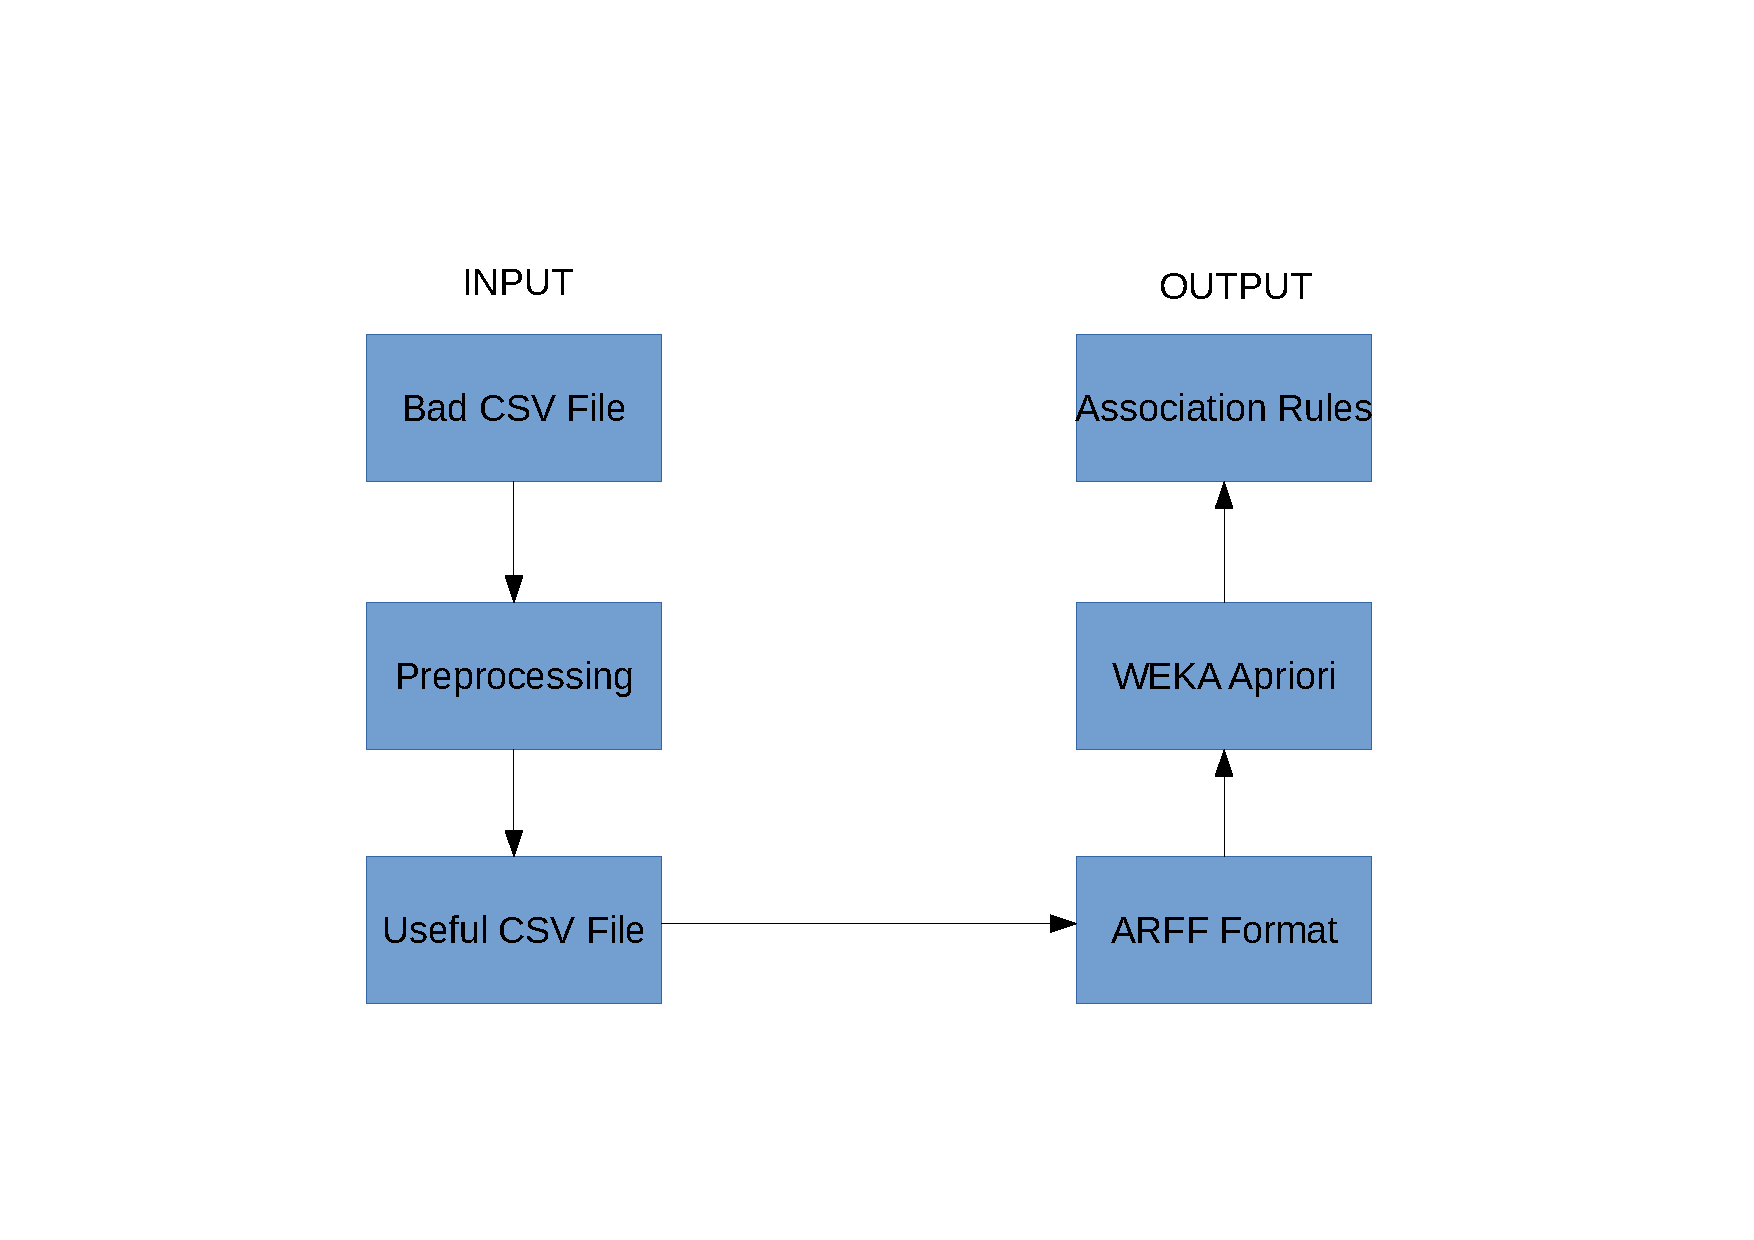
\includegraphics[height=3in,width=4.5in]{abbildungen/approachpdf.pdf}
		\caption{Steps of the used mining process}
			\label{fig:roughapproach}
	\end{center}
\end{figure}

\begin{description}
	\item[Bad CSV-file]\hfill \\
	All heating data is stored in form of CSV-files. Producing this data was not part of this work and should be credited to ENER-IQ. The types of CSV-files at hand were explained in section \ref{sec:preprocessing}.
	\item[Preprocessing]\hfill \\ 
	In this step, strategies discussed in section \ref{sec:strategies} are applied to generate different presets. In order to do so, CSV Preprocessing in Java via its Prolog interface is applied.
	\item[Useful CSV-file]\hfill \\ 
	The output of the Preprocessing step.
	\item[ARFF Format]\hfill \\ 
	The preprocessed useful CSV-files are converted to ARFF files, which are the necessary input files for WEKA Apriori, via the Declare framework in Prolog.	
	\item[WEKA Apriori]\hfill \\ 
	The converted ARFF-file, together with WEKA Apriori execution parameters explained in section \ref{sec:wekaapriori}, are used to mine association rules and frequent itemsets. This is the main execution procedure.
	\item[Association Rules]\hfill \\ 
	The Declare framework outputs the association rules generated by WEKA Apriori into a text file, which is the end result of the process. As often in association rule mining, the evaluation of association rules are mostly done manually. Chapter \ref{sec:relatedwork} explains, why metrics, such as \textit{precision} or \textit{accuracy} could not be used in this approach.
	
\end{description}



\chapter{Implementation}
\label{sec:implementation}

This chapter lays out the implementation used for the experiments in \ref{sec:evaluation}.

The general structures consists of an implementation of Equal-Width Discretization in Java, a Prolog wrapper, and experiments utilizing the Prolog wrapper.


\section{CSV-Preprocessor in Java}

The methods \textit{substringFrom} and \textit{processSubstringTable} in \ref{lst:substringingimpl} are called, when the Prolog wrapper sends a substringing command.

	\begin{lstlisting}[language=java, caption= Implementation substringing in Preprocessor.java, label={lst:substringingimpl}]
public String substringFrom(String s, int a, int b)
{
	String sub = s.substring(Math.min(a, s.length()), Math.min(s.length(), b));
	return sub;
}


public void processSubstringTable(int column, int a, int b)
{
	for(int i = 0; i < table.size(); i++)
	{
		table.get(i).set(column, substringFrom(table.get(i).get(column), a, b));
	}
}
	\end{lstlisting}
	
	
The same concept in substringing applies for bucketing - which implements the main part of the Equal-Width Discretization - and constructing new columns, as seen in \ref{lst:bucketingimpl} and \ref{lst:constructingimpl}

	\begin{lstlisting}[language=java, caption= Implementation substringing in Preprocessor.java, label={lst:bucketingimpl}]
public void processIntervalTable(int column, int intervals)
{
	double min = Double.valueOf(table.get(1).get(column));
	double max = Double.valueOf(table.get(1).get(column));
	for(int i = 0; i < table.size(); i++)
	{
		double currEntry = Double.valueOf(table.get(i).get(column));
		if(currEntry > max) max=currEntry;
		if(currEntry < min) min=currEntry;
	}
	double intervalsize = (max - min)/intervals;
	for(int i = 0; i < table.size(); i++)
	{
		double currStart = min;
		double currEntry = Double.valueOf(table.get(i).get(column));
		while(currEntry > currStart + intervalsize)
		{
			currStart += intervalsize;
		}

		table.get(i).set(column, String.format("%f to %f", currStart, (currStart+intervalsize)));
	}

}
\end{lstlisting}

	\begin{lstlisting}[language=java, caption= Implementation substringing in Preprocessor.java, label={lst:constructingimpl}]
public void constructNewColumn(String name, int index1, int index2, int code)
{
	header.add(name);
	table.get(0).add(name);
	int amountRows = table.size();


	double left;
	double right;
	for(int i = 0; i < amountRows; i++)
	{
		left = Double.parseDouble(table.get(i).get(index1));
		right = Double.parseDouble(table.get(i).get(index2));
		switch(code)
		{
			case DIFFERENCE:
				table.get(i).add(String.valueOf(left - right));
				break;

			case SUM:
				table.get(i).add(String.valueOf(left + right));
				break;

			case PRODUCT:
				table.get(i).add(String.valueOf(left * right));
				break;

			case DIVISION:
				table.get(i).add(String.valueOf(left / right));
				break;
		}
	}
}
\end{lstlisting}

\section{CSV-Preprocessor wrapper in Prolog}

Listing \ref{lst:wrapperimpl} implements a wrapper in Prolog for the aforementioned preprocessing functions in Java.

\begin{lstlisting}[language=Prolog, caption= Implementation of wrapper predicates in Prolog, label={lst:wrapperimpl}]
csv_process_substring(Input, Column, From, To, Output) :-
atomic_list_concat(['java -jar /home/thebrocc/Desktop/CSVPreprocessor.jar', Input, 'substring', Column, From, To, Output], ' ' , Command),
shell(Command).

csv_process_bucketing(Input, Column, Buckets, Output) :-
atomic_list_concat(['java -jar /home/thebrocc/Desktop/CSVPreprocessor.jar', Input, 'bucketing', Column, Buckets, Output], ' ' , Command),
shell(Command).

csv_process_construct(Input, Column1, Column2, Operator, Name, Output) :-
atomic_list_concat(['java -jar /home/thebrocc/Desktop/CSVPreprocessor.jar', Input, 'construct', Column1, Column2, Operator, Name, Output], ' ' , Command),
shell(Command).
\end{lstlisting}

Ultimately, the predicate that is called on a given CSV-file, which applies WEKA-Apriori and outputs association rules, is implemented in \ref{lst:rules}.


\begin{lstlisting}[language=Prolog, caption= Implementation of predicate which generates association rules from CSV-files in Prolog, label={lst:rules}]
csv_to_association_rules(Inputfile, Table_Name, Attributes, Parameters) :-
csv_read_file(Inputfile, Rows, []),
csv_rows_to_lists(Rows, [_|UsefulRows]),
weka_association_rules_parametrized(Table_Name, Attributes, UsefulRows, Rules, Parameters).
\end{lstlisting}

\section{Implementation of experiments}
Experiments use the aforementioned predicates of the wrapper in Prolog. Experiment \ref{lst:hk1experiment} is an example of usage. Here, \textit{hk1.csv} is processed into \textit{hk1preprocessed.csv} using the wrapper predicates.


\begin{lstlisting}[language=Prolog, caption= Implementation of heating preprocessing, label={lst:hk1experiment}]
run_preprocess_heating(Buckets) :-
csv_process_substring('/home/thebrocc/Desktop/Heizungsdaten/Heating/hk1.csv', 0, 0, 15, '/home/thebrocc/Desktop/Heizungsdaten/Preprocessed/Heating/hk1first.csv'),
csv_process_construct('/home/thebrocc/Desktop/Heizungsdaten/Preprocessed/Heating/hk1first.csv', 2, 3, 'sub', 'spreizung', '/home/thebrocc/Desktop/Heizungsdaten/Preprocessed/Heating/hk1second.csv'),
csv_process_bucketing('/home/thebrocc/Desktop/Heizungsdaten/Preprocessed/Heating/hk1second.csv', 1, Buckets, '/home/thebrocc/Desktop/Heizungsdaten/Preprocessed/Heating/hk1third.csv'),
csv_process_bucketing('/home/thebrocc/Desktop/Heizungsdaten/Preprocessed/Heating/hk1third.csv', 2, Buckets, '/home/thebrocc/Desktop/Heizungsdaten/Preprocessed/Heating/hk1fourth.csv'),
csv_process_bucketing('/home/thebrocc/Desktop/Heizungsdaten/Preprocessed/Heating/hk1fourth.csv', 3, Buckets, '/home/thebrocc/Desktop/Heizungsdaten/Preprocessed/Heating/hk1fifth.csv'),
csv_process_bucketing('/home/thebrocc/Desktop/Heizungsdaten/Preprocessed/Heating/hk1fifth.csv', 4, Buckets, '/home/thebrocc/Desktop/Heizungsdaten/Preprocessed/Heating/hk1preprocessed.csv')
\end{lstlisting}

After generating preprocessed CSV-files \ref{lst:execute} illustrates, how a preprocessed file is used to run differently parametrized experiments.


\begin{lstlisting}[language=Prolog, caption= Running parametrized experiments, label={lst:execute}]
run_experiment_1(TableName, Bucketsize, Parameters) :-
atomic_list_concat(['/home/thebrocc/Desktop/Heizungsdaten/Preprocessed_20k_', Bucketsize, 'Buckets/Heating/hk1preprocessed.csv'], '' , Path),
csv_to_association_rules(Path, TableName, [zeitpunkt, aussentemp, vorlauf, ruecklauf, spreizung] , Parameters).
\end{lstlisting}

\section{Declare}

Some minor changes had to be added to Declare in order to be able to run parametrized experiments. The predicates \texttt{weka\_association\_rules} and \texttt{weka\_associations\_file} responsible for applying WEKA on a table had to be extended to allow for dynamic WEKA parameters, as seen in \ref{lst:declarechanged}

\begin{lstlisting}[language=Prolog, caption= Slightly extended predicates in the weka wrapper of Declare, label={lst:declarechanged}]
weka_association_rules_parametrized(Table_Name, Rules, Parameters) :-
data_mining_table_2(Table_Name, Attributes, Rows),
weka_association_rules(Table_Name, Attributes, Rows, Rules_2, Parameters),
weka_association_rules_transform(Rules_2, Rules),
dwrite(xml, Rules).

weka_association_rules_parametrized(Table_Name, Attributes, Rows, Rules, Parameters) :-
table_rows_prune_for_weka(Rows, Rows_2),
dislog_variable_get(output_path, 'weka_input.arff', File_In),
table_to_weka_file(Table_Name, Attributes, Rows_2, File_In),
dislog_variable_get(output_path, 'weka_output', File_Out),
weka_associations_file(File_In, File_Out, Parameters),
weka_file_to_rules(File_Out, Rules),
!.

weka_associations_file(File_In, File_Out, Parameters) :-
concat([ 'cp ', File_In,
' /home/thebrocc/Weka/data/weka_input.arff' ],
Cp_Command_1),
writeln(user, Cp_Command_1),
us(Cp_Command_1),
concat([ 'cd /home/thebrocc/Weka; ',
'java -cp ./weka-3_6_0.jar weka.associations.Apriori -t data/weka_input.arff ', Parameters, ' > data/weka_output' ],
Command),
writeln(user, Command),
us(Command),
concat([ 'cp',
' /home/thebrocc/Weka/data/weka_output ',
File_Out ], Cp_Command_2),
writeln(user, Cp_Command_2),
us(Cp_Command_2).
\end{lstlisting}







\chapter{Experiments and Evaluation}
\label{sec:evaluation}
The following chapter is concerned with evaluating different preprocessing presets and the generation of association rules under different sets of WEKA Apriori parameters with the goal of finding rules, which reflect known or realistic phenomenons in heating circuits. In this regard, a strategy is considered better than another if it allows us to mine said rules. This chapter is split into two parts; the first part suggesting multiple preprocessing presets using the CSV-Preprocessor introduced in the previous chapter, whereas in the second part we try to evaluate the impact of WEKA-Apriori parameters on the quality of the resulting association rules.


\section{Dealing with nominal value columns}
\label{sec:nominalvalues}

We know that any given \textit{Uhrzeit} item consists of the same amount of characters, each character position representing the exact same information. Therefore, using a substring from indeces 0 to 10 on an \textit{Uhrzeit} item should return it formatted to YYYY-MM-DD. Since measurements were carried out in minutely intervals, the hypothesis here should be that enough measurements per day were carried out in order for the Uhrzeit attribute to appear in frequent itemsets, which previously wasn't the case. However, an hourly recurring pattern between the measured temperatures should be visible. Due to this feedback, the following presets used substringing from indices 0 to 15, formatting every date to YYYY-MM-DD-hh. 
We have to remember that simply cutting off a date string at any arbitrary point results in information loss. Deciding whether we should format a date leaving out only the minutes or leaving out both hours and minutes is dependent on how sensitive this information is. Here, feedback of domain specific experts is important.

In order to trim the date attribute, \texttt{csv\_process\_substring(Input, Column, From, To, Output)} was used.



\section{Dealing with floating point value columns}
\label{sec:floatingpointvalues}
For the sake of simplicity, Equal-Width Discretization for temperature data has been chosen. Each original CSV-File has been transformed into four different preprocessed files (2 buckets, 5 buckets, 8 buckets, 10 buckets). For this, predicate \texttt{csv\_process\_bucketing(Input, Column, Buckets, Output)} - which is called in the \texttt{csv\_process\_X(Input, Column, Buckets, Output)} predicates -  was used. The amount of buckets have been chosen through manual interval cascading, after first experimenting with 2 and 10 buckets, which has shown to yield either too vague or too concrete rules. The conclusion was, that an ideal discretization would have been between 2 buckets and 10 buckets.

\section{Comparison of amount of itemsets and rules extracted}
\label{sec:amountofrules}

In order to gain a rough overview of the mined rules, one generator, heater, and hotwater CSV-File were mined under the same parameters. The parameters chosen are mostly standard, however aren't too relevant when comparing the amount of rules mined relative to each generator/heater/hotwater file (N=4000, C=0.01). The most important point of interest however is the amount of rules mined compared to the different amount of bucket presets (0, 2, 5, 8, 10). The amount of rules relative to each other is plotted in figure \ref{fig:amountofrules}. As already known, at 0 Buckets, which indicates no discretization, no rules are mined. Starting from 2 buckets we can see a monotone downward trend for all files, except for Hotwater 1. The hypothesis for the latter is that there is a measurement error in the hotwater file, since further investigation has shown temperatures in the quadruple digits in the negative (which shouldn't be possible and is likely the reason for the anomaly). 
At 10 buckets the amount of rules mined come to a minimum. This is due to intervals being more narrow and therefore the probability for a given itemset to frequent is less likely. The more buckets are used for discretization, the closer the results are to using 0 buckets, since the maximum amount of buckets is equal to using a bucket for every value which is equal to no buckets at all.
At 2 buckets the amount of rules come to a maximum, which is due to the buckets being larger, and the opposite effect occurs. However, the rules mined become so vague that only trivial conclusions can be made, such as "when flow temperature lands in the upper bucket, return temperature lands in the lower bucket" which essentially only describes that a heater radiates energy, which in return cools down water.

Figure \ref{fig:itemsetsizes} illustrates that large itemsets are most frequent with 5 or 8 buckets, which again indicates that 5 or 8 buckets should be the most rewarding discretization.

\begin{figure}[htb]
	\begin{center}
		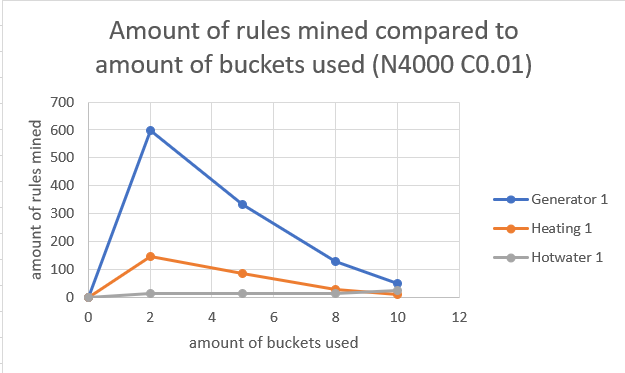
\includegraphics[scale=0.65]{abbildungen/amountofrules.PNG}
		\caption{Comparison of amount of rules mined}
			\label{fig:amountofrules}
	\end{center}
\end{figure}

\begin{figure}[htb]
	\begin{center}
		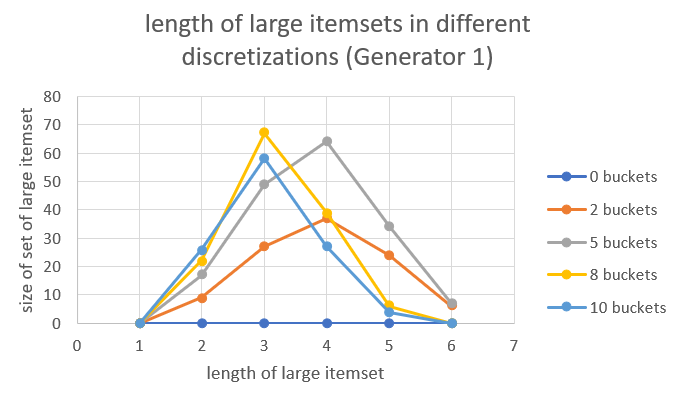
\includegraphics[scale=0.65]{abbildungen/itemsetssize.PNG}
		\caption{Comparison of mined itemsets}
			\label{fig:itemsetsizes}
	\end{center}
\end{figure}

\section{Comparing different preprocessing presets on the same heater}
\label{sec:sameheater}
In order to extract knowledge from a specific heater (\textit{hk1} or \textit{Heating 1}), WEKA-Apriori has been applied to the same preprocessed CSV-file. Since we concluded that discretization with 5 or 8 buckets should be more rewarding, the focus will be on these presets. Another variable which hs been ignored so far are WEKA parameters, as explained in section \ref{sec:wekaapriori}. The different parameter presets here are \textit{N 100 C 0.01}, \textit{N 4000 C 0.01}, \textit{N 4000 C 0.01 M 0.05}.

The disappointing trend in all of the results is, that most rules are a representation of the same piece of information. For example, the best rule on preset \textit{N 100 C 0.01} with 5 buckets is the following:

\begin{lstlisting}[style=arff, caption=best rule from N 100 C 0.01 - 5 buckets]
1. aussentemp=12.000000 to 16.600000 vorlauf=58.040000 to 65.920000 spreizung=25.000000 to 37.200000 2383 ==> ruecklauf=29.400000 to 36.200000 2348    conf:(0.99)
\end{lstlisting}


The interpretation of this rule is trivial: When the outside temperature is rather low (12\textcelsius to 16\textcelsius), and flow temperature is rather high (58\textcelsius  to 66\textcelsius), the spread  between flow and return temperature is high (25\textcelsius  to 37\textcelsius), our return temperature is almost always (0.99 confidence) low (29.4\textcelsius  to 36\textcelsius). This makes sense, since a lower outside temperature allows for the heater to radiate a larger amount of its energy. This is also the reason the difference between flow and return temperature is rather high, and the fact that flow temperature is almost always higher than return temperature is also trivial. That means, that we might expect a lower difference between flow and return, when the outside temperature is higher. This could not be shown, due to the outside temperature rarely being higher than 21\textcelsius. We have to remember that the difference of flow and return might be also dependent on variables we don't have access to, such as the type and size of the pipes which the heated water flows through or the type of radiator. For example, we might expect a radiator with a larger surface to radiate more energy  than a radiator of smaller size. One could use the extracted rule of a higher average spread between return and flow to determine what kind of heater was used as some sort of classification, but its not conclusive whether this would be due to a fault or e.g. a specific type of radiator that is known for radiating less energy.


Another trend is that the artificially constructed column \textit{Spreizung} has not been proven useful, since it floods the output with redundant rules - once including all three attributes from \textit{Spreizung, Vorlauf, Rücklauf} and once only including two of them. Here we are reminded of the prior definition of data mining, which attempts to extract "hidden knowledge" from a given data set. Since \textit{Spreizung} is generated from already known information, no new information is extracted. However, it can help with human readability.

The following example shows three rules almost identical in meaning.

\begin{lstlisting}[style=arff, caption=redundant rules in N 100 C 0.01 M 0.05]
1. aussentemp=12.000000 to 16.600000 vorlauf=58.040000 to 65.920000 spreizung=25.000000 to 37.200000 2383 ==> ruecklauf=29.400000 to 36.200000 2348    conf:(0.99)
  
2. aussentemp=12.000000 to 16.600000 spreizung=25.000000 to 37.200000 2475 ==> ruecklauf=29.400000 to 36.200000 2438    conf:(0.99)

3. spreizung=25.000000 to 37.200000 5429 ==> vorlauf=58.040000 to 65.920000 5318    conf:(0.98)
\end{lstlisting}

When looking into the output of the same preset and 8 buckets, one can observe that the rule stating that a low outside temperature causes a high difference in flow and return does not appear anymore. This information loss is due to the buckets being too narrow. The difference between \textit{N 100 C 0.01} and \textit{N 4000 C 0.01} is almost non existent due to not enough rules being generated for the parameter \textit{N} to make a difference. However, a significant difference between preset \textit{N 4000 C 0.01} and \textit{N 4000 C 0.01 M 0.05} can be seen, mainly the addition of rules with very low confidence values, which can be either interpreted as outliers or anomalies.



\section{Attempting to extract knowledge regarding anomalies}
\label{sec:extractinganomalies}
One issue with mining knowledge regarding anomalies is the fact that this approach is based on frequent itemset mining. It is difficult to distinguish a regular outlier from actual anomalies that indicates faults. One attempt might be lowering both minimum confidence and the minimum lower bound for support parameters to make outliers at least appear in the output files, but even then the mined rules become hyper specific and questionable due to the low confidence value. This is shown in section \ref{sec:extractingtime} when attempting to extract knowledge regarding the \textit{Uhrzeit} attribute.
Again, observable anomalies are rather trivial, as shown by the following rule:


\begin{lstlisting}[style=arff, caption=rule indicating irregular behavior]
194. vorlauf=58.040000 to 65.920000 8998 ==> spreizung=0.600000 to 12.800000 1155    conf:(0.13)
\end{lstlisting}

This indicates that flow and return temperature are approximate, which should rarely be the case (confidence 0.13), because that would mean that the radiator is not able to radiate its energy.

Another worthy point of mention is that the engineers claimed that the data at hand is almost free of anomalies and should mostly show regular procedures of heating circuits.

\section{Comparing rules mined under differently prioritized metrics}
\label{sec:sorting}
In theory, when setting the WEKA parameter \textit{T}, the output should be sorted by either confidence (T=0), lift (T=1), leverage (T=2), or conviction (T=3). For example, sorting by lift should highlight more significant rules, while sorting by conviction should highlight rules where the conclusion is highly dependent on their left side. However, due to the mined rules being mostly redundant, the output is very similar - no matter how the rules are sorted. Have in mind that the rules and itemsets are the same, but differently sorted for human highlighting.

\section{Attempting to extract knowledge regarding time}
\label{sec:extractingtime}

One obvious takeaway from the previous experiments are that the attribute \textit{Uhrzeit} didn't appear in frequent itemsets once. The hypothesis here is that the WEKA parameter for minimum support threshold  weeds out all appearances of \textit{Uhrzeit}. This is proven when lowering the parameter \textit{M} to 0.01 and applying \textit{run\_experiment\_time\_hk1(Index)}: The newly generated rules' itemsets contain the \textit{Uhrzeit} attribute, however due to the minimum support threshold being trivially low, the mined rules are meaningless.




\chapter{Future work}
\label{sec:futurework}
The presented approach is one very specific implementation of discretization data. However, it is possible that different approaches deliver better results, such as Equal-Frequency-Discretization \cite{jiang2009approximate}. Another major point of improvement is the user friendliness of the preprocessing framework being used. While currently a new file has to be generated for discretizing each column, a future implementation could send all preprocessing instructions via JSON-file and take a single JSON-file as an input, which would also improve the performance as it would reduce the load of writing data into files. Another way of improving the quality of rules are adding more attributes into the data mining process. For example, one could imagine that the size and type of the pipes would also be a factor in determining whether the amount of energy radiated is appropriate or not.


\chapter{Summary}
\label{sec:summary}
In this study, a given set of heating systems data has been preprocessed using an implementation of Equal-Width Discretization and substringing. By analyzing the itemsets generated under different discretization parameters, a preprocessed set of data has been chosen and data mining through WEKA-Apriori has been applied. The results were rather vague but helpful in provided an overview of the heating systems at hand. While most of the mined rules were redundant, trivial conclusions can be made, such as water in the pipes cooling down after arriving at the radiator. This is also useful in detecting rough faults, such as the heater not radiating enough energy, despite the flow temperature being high and the outside temperature being low. Still, more attributes, such as type and size of radiator and pipes, used in the mining processed could be helpful in extracting more specific and conclusive knowledge, rather than a broad overview. Another conclusion is that proper data preprocessing heavily outweighs choosing effective WEKA parameters and choosing a low \textit{M} and \textit{C} parameter could be helpful in finding anomalies.

The abnormally low and high temperatures shown in the hotwater CSV-files has also shown a major weakness in this implementation of Equal-Width Discretization: Infrequent spikes in measurements can cause too large buckets and make any conclusion meaningless. Here, Equal-Frequency Discretization could be useful.






%%%%%%%%%%%%%%%%%%%%%%%%%%%%%%%%%%%%%%%%%%%%%%%%%%%%%%%%%%%%%%%%%%%%%%%%%%%%%%%%
%%% Literaturverzeichnis
\thesisbibliography
\bibliography{mybib}





%%%%%%%%%%%%%%%%%%%%%%%%%%%%%%%%%%%%%%%%%%%%%%%%%%%%%%%%%%%%%%%%%%%%%%%%%%%%%%%%
%\appendix




\end{document}
